% \documentclass[aspectratio=169,notes]{beamer}
\documentclass[aspectratio=169]{beamer}
\usetheme[faculty=phil]{fibeamer}
\usepackage{polyglossia}
\setmainlanguage{english} %% main locale instead of `english`, you
%% can typeset the presentation in either Czech or Slovak,
%% respectively.
\setotherlanguages{russian} %% The additional keys allow
%%
%%   \begin{otherlanguage}{czech}   ... \end{otherlanguage}
%%   \begin{otherlanguage}{slovak}  ... \end{otherlanguage}
%%
%% These macros specify information about the presentation
\title[MaM]{Mechanics and Machines, HW CAE DYN 1} %% that will be typeset on the
\subtitle{Inverse Dynamics Problem
\\ \  \\ \ 
         } %% title page.
\author{Oleg Bulichev}
%% These additional packages are used within the document:
\usepackage{ragged2e}  % `\justifying` text
\usepackage{booktabs}  % Tables
\usepackage{tabularx}
\usepackage{tikz}      % Diagrams
\usetikzlibrary{calc, shapes, backgrounds}
\usepackage{amsmath, amssymb}
\usepackage{url}       % `\url`s
\usepackage{listings}  % Code listings
% \usepackage{subfigure}
\usepackage{floatrow}
\usepackage{subcaption}
\usepackage{mathtools}
\usepackage{todonotes}
\usepackage{fontspec}
\usepackage{multicol}
\usepackage{pdfpages}
\usepackage{wrapfig}
\usepackage{animate}
\usepackage{booktabs}
\usepackage{multirow}
% \usepackage{graphicx}
\usepackage{colortbl}

\graphicspath{{resources/}}
\frenchspacing

\setbeamertemplate{caption}[numbered]
\usetikzlibrary{graphs}

% \usepackage[backend=biber,style=ieee,autocite=footnote]{biblatex}
% \addbibresource{biblio.bib}
% \DefineBibliographyStrings{english}{%
%   bibliography = {References},}

\newcommand{\oleg}[2][] {\todo[color=red, #1] {OLEG:\\ #2}}
\newcommand{\fbckg}[1]{\usebackgroundtemplate{\includegraphics[width=\paperwidth]{#1}}}%frame background

\usepackage[framemethod=TikZ]{mdframed}
\newcommand{\dbox}[1]{
\begin{mdframed}[roundcorner=3pt, backgroundcolor=yellow, linewidth=0]
\vspace{1mm}
{#1}
\vspace{1mm}
\end{mdframed}
}

\begin{document}
\setlength{\abovedisplayskip}{0pt}
\setlength{\belowdisplayskip}{0pt}
\setlength{\abovedisplayshortskip}{0pt}
\setlength{\belowdisplayshortskip}{0pt}

\fbckg{fibeamer/figs/title_page.png}
\frame[c]{\setcounter{framenumber}{0}
    \usebeamerfont{title}%
    \usebeamercolor[fg]{title}%
    \begin{minipage}[b][6.5\baselineskip][b]{\textwidth}%
        \textcolor{black}{\raggedright\inserttitle}
    \end{minipage}
    % \vskip-1.5\baselineskip

    \usebeamerfont{subtitle}%
    \usebeamercolor[fg]{framesubtitle}%
    \begin{minipage}[b][3\baselineskip][b]{\textwidth}
        \raggedright%
        \insertsubtitle%
    \end{minipage}
    \vskip.25\baselineskip
}
%   \frame[c]{\maketitle}

\fbckg{fibeamer/figs/common.png}

\note{\scriptsize \begin{itemize}
        \item \
    \end{itemize}}

\note{
   \ 
}

\begin{frame}[t]{Short Task Description}
    \framesubtitle{}
    \textbf{Description}: Solve Inverse Dynamics problem for four link bar mechanism by coding and by NX Motion Analysis application.

    \textbf{Artifacts}: 
    \begin{itemize}
        \item Zip archive with NX detail files (.prt) and simulation (.sim)
        \item Code, which can be executed anywhere
        \item 1-3 pages report in (.pdf). It should contain formulas, explanation, considered assumptions and results.
    \end{itemize}
\end{frame}

\begin{frame}[t]{Extended Task Description}
\framesubtitle{}
\vspace{-0.6cm}
    \begin{columns}[T,onlytextwidth]
        \begin{column}{0.59\textwidth}
            \scriptsize
    \textbf{Zip archive, which contains all needed data}: \textit{HWs/HW\_CAE\_DYN1/task\_data}
    
    1st joint is controllable, others --- not.
    \vspace{-0.1cm}
    \begin{enumerate}
        \item \textbf{Find angle limits} (where the mechanism stuck) for controllable joint:
        \vspace{-0.45cm}

        \begin{itemize}
            \scriptsize
            \item By code (solving kinematics problem for each angle)
            \item Using NX (either Modeling, or Animation Designer);
        \end{itemize}
        \vspace{-0.2cm}

        \item Compare results, present them as a pie chart in report.
        \item \textbf{Make the scene in Motion Analysis}. All links are made from <<Bronze>>. You need to add joints, contacts, direct earth gravity correctly.
        \item Choose the biggest angle gap between joint limits and put your link in the beginning of it.
        \item Apply constant angular acceleration for 1st joint --- 0.2 $rad / s^2$
        \item \textbf{Find a torque for 1st joint} for such angle gap:
        \vspace{-0.1cm}

        \begin{itemize}
            \scriptsize
            \item By code (solving Inverse dynamics problem)
            \item Using NX (any solver);
        \end{itemize}
        \vspace{-0.2cm}

        \item Compare results
    \end{enumerate}
        \end{column}
        \begin{column}{0.39\textwidth}
            \vspace{1cm}
            \begin{figure}[H]
                \centering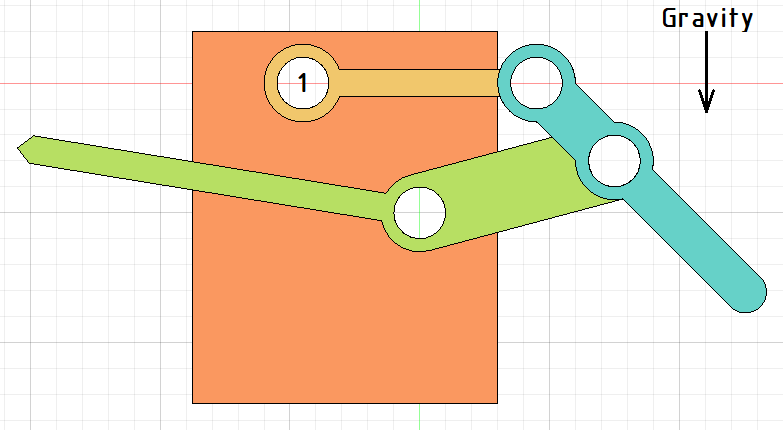
\includegraphics[height=6cm,width=1\textwidth,keepaspectratio]{task_descr.png}
                % \caption{caption_name}
                \label{fig:task_descr.png}
            \end{figure}
        \end{column}
    \end{columns}
\end{frame}


\fbckg{fibeamer/figs/last_page.png}
\frame[plain]{}

\end{document}